%!TEX root = ../thesis.tex

\section{背景}
AI-Formulaは計測自動制御学会と自動車技術会が主催し, 本田技術研究所がサポートする自律移動モビリティの競技会で, 正式な競技会は2025年から始まる. \cite{AI-Formula}
AI-Formulaはスピードと知能を競うリアルワールドレースであり, 次世代モビリティに必要な技術を身につける機会を提供し, 自動化システムのエンジニアを育成することを一つの目的としている.
%
実環境でモビリティを自律走行させてレースを行うため, ハードウェアとソフトウェアの両方が要求される.
しかし, AI-Formulaではハードウェアは貸与の形式で与えらているため, 現時点での開発はソフトウェアの開発が主となる.
ハードウェアは経路追従するために必要なパーツが全て揃っているが, ソフトウェアはモビリティを制御するためのシステムの基盤となるベースソフトウェアが用意されているのみである. \cite{AI-Formula-support}
そのため, 経路追従などのソフトウェアは各チームで開発することが必要となる.
\cite{AIFormula-chibakou} \cite{AIFormula-repo}


\subsection{ハードウェア}
AI-Formulaでは詳細なルールは検討中であるとのことで, 2025年3月に開催される予定のプレ大会以降に詳細なルールが決定される予定となっている.
Fig.1.1に2025年のプレ大会で使用される予定のモビリティを示す.
AI-Formulaでは, モビリティは本田技術研究所から貸与される.
貸与されたモビリティは差動二輪と一輪のキャスタ(以下, 従動輪と呼ぶ)で構成された三輪モデルである.
貸与されたモビリティには, ステレオカメラ(ZED-X stereolabs)やGNSS+IMUセンサ(VN-200 VectorNav)が搭載されている.
バッテリーにはMPP(Mobile Power Pack)が使用される. MPPは持ち運び可能な交換式バッテリーとなっている. Fig.1.2にMPPを示す.
% MPPをセンサの画像に差し替える
% モビリティのセンサの位置を示す画像にする or センサ単品の画像を2つ
プレ大会では指定されたコースを3周する時間で競う予定となっている.

\begin{figure}[H]
  \centering
 \includegraphics[keepaspectratio, scale=0.6]
      {images/ExteriorViewOfTheMobilityPlatform.png}
 \caption{Exterior view of the mobility platform}
 \label{fig:robot view}
\end{figure}

\begin{figure}[H]
  \centering
 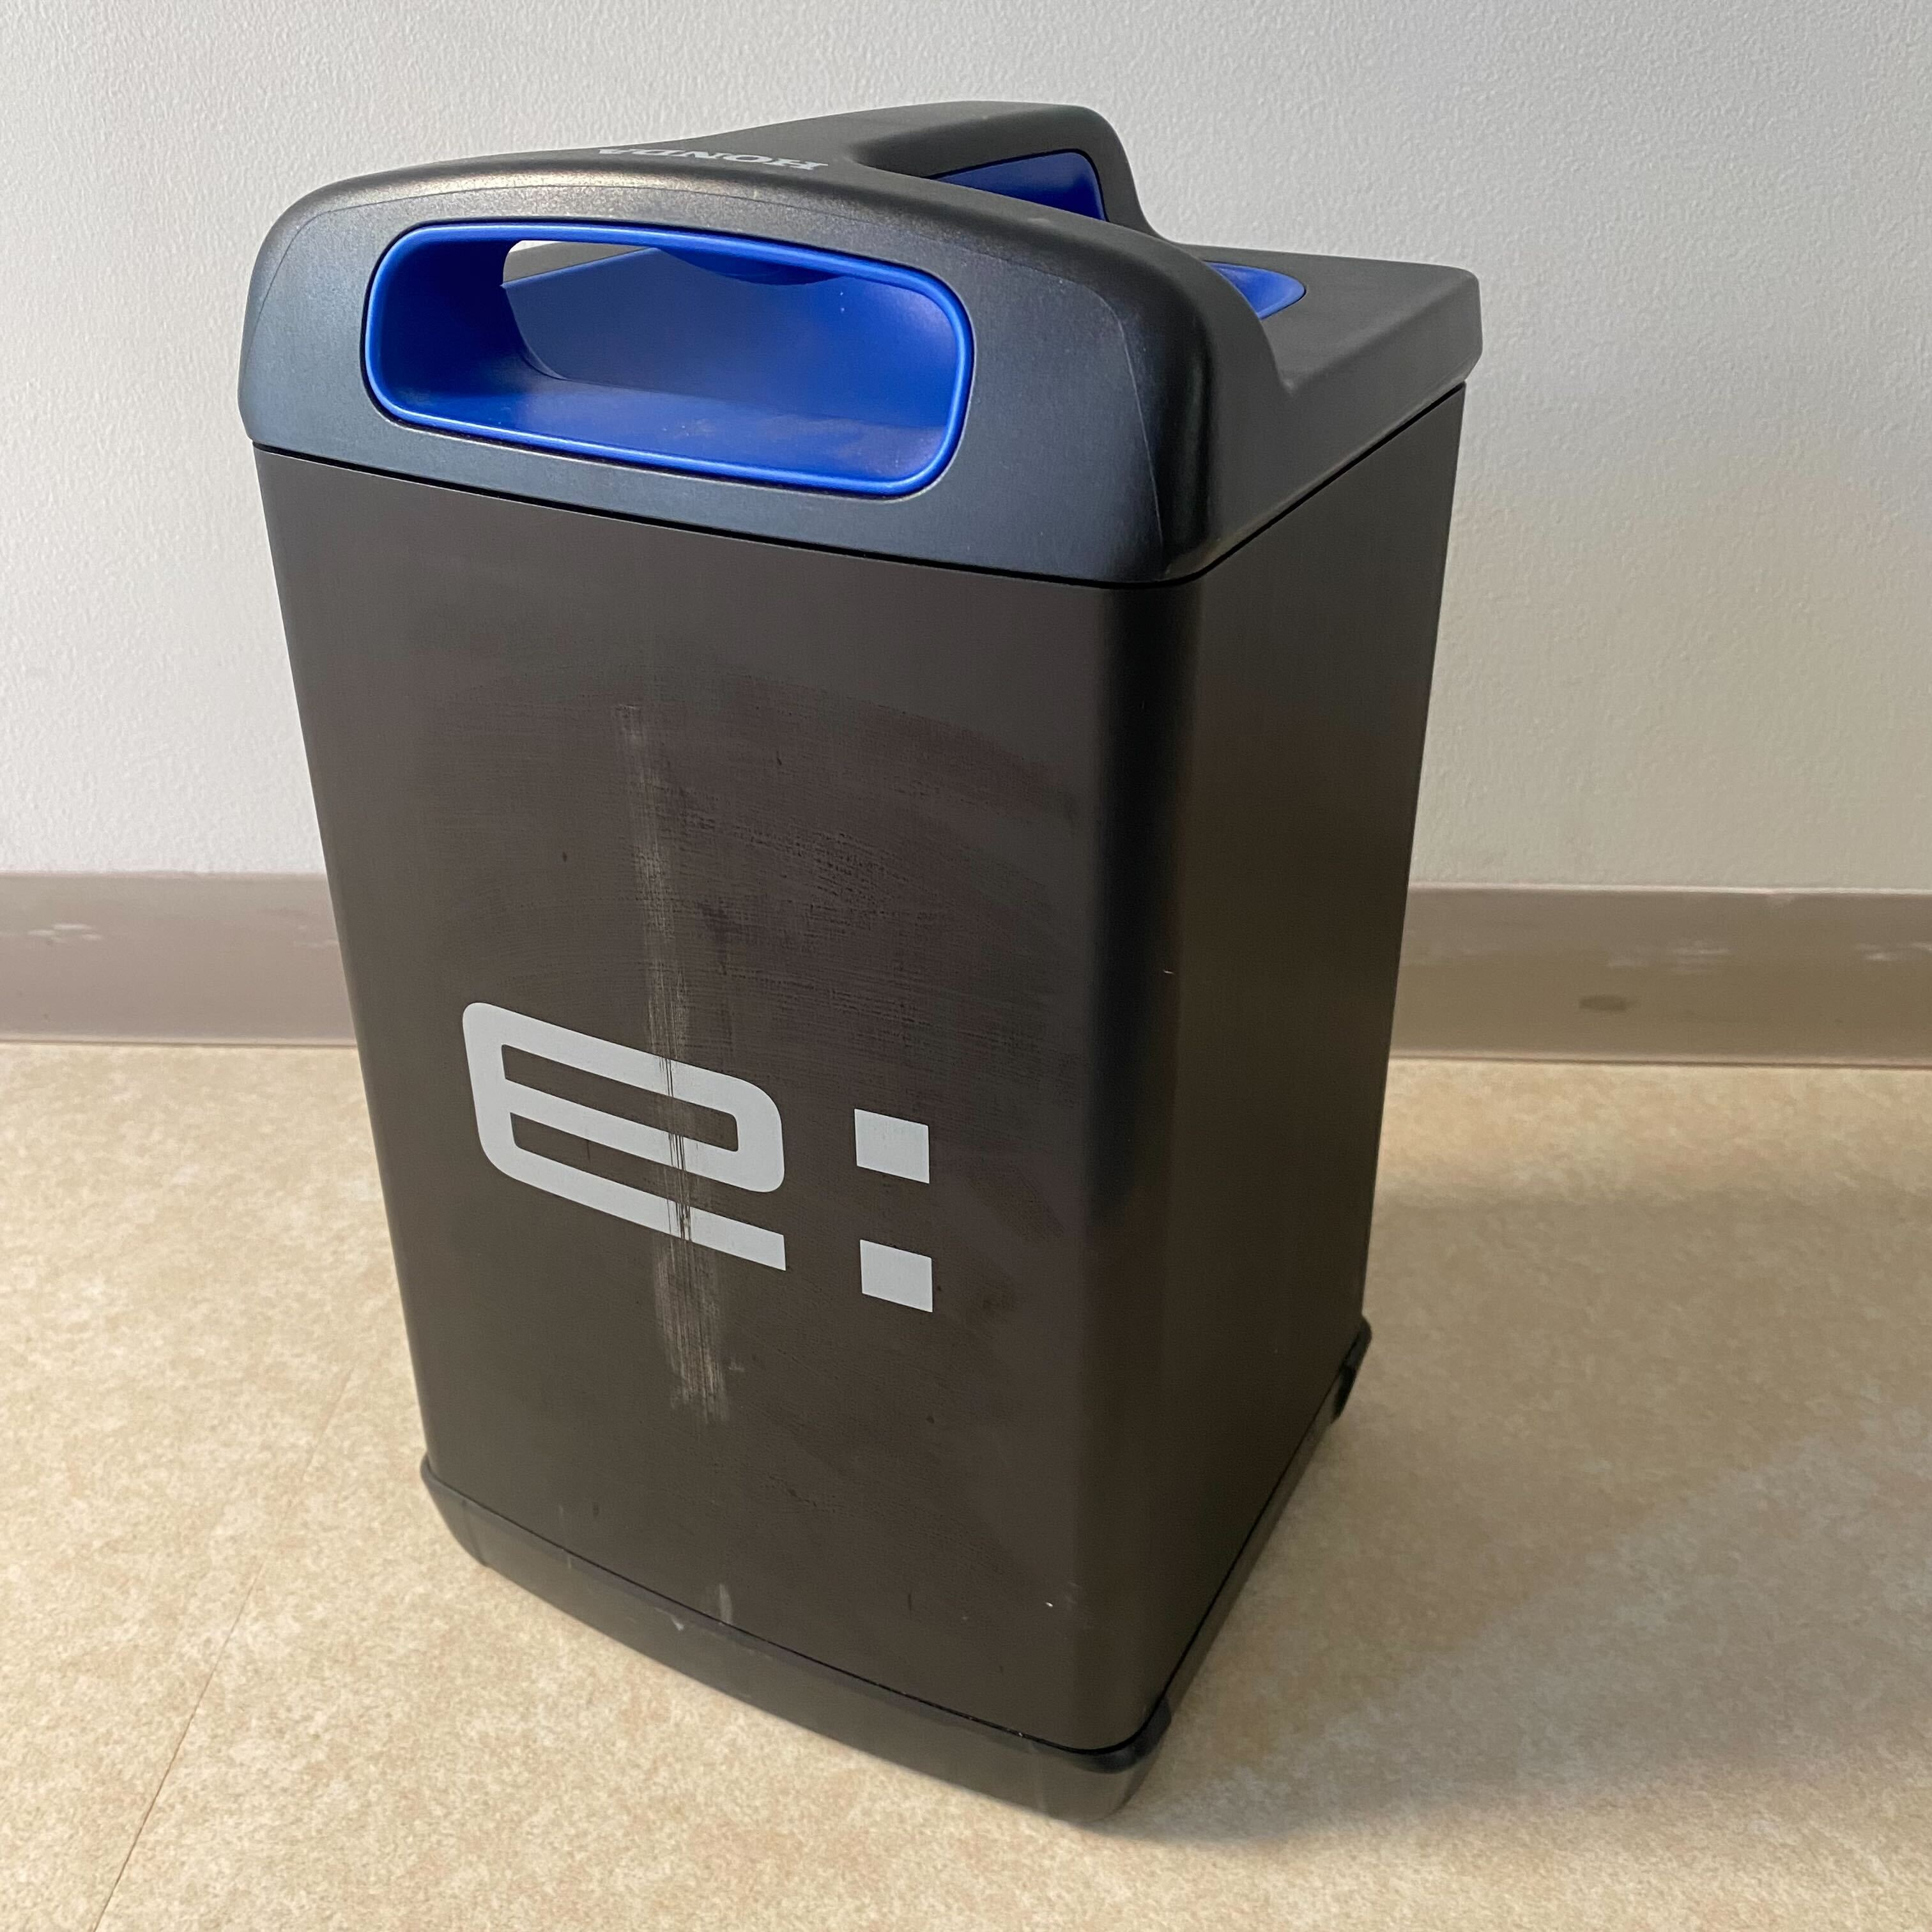
\includegraphics[keepaspectratio, scale=0.08]
      {images/mpp.png}
 \caption{Mobile Power Pack}
 \label{fig:MPP}
\end{figure}

\subsection{コース}
AI-Formulaのコンテストは, 茨城県常総市に位置するAIモビリティパーク紫峰において実施される.
AIモビリティパーク紫峰はアスファルト舗装された路面や車線などの路面情報が整備されているコースである.
Fig.1.3にAIモビリティパーク紫峰を示す.

% コース全体図じゃなくて地上からの写真でも良いかも
\begin{figure}[H]
  \centering
 \includegraphics[keepaspectratio, scale=0.1]
      {images/realworld.png}
 \caption{AI-Formula Course}
 \label{fig:course}
\end{figure}


\section{目的}
本研究では, 屋外自律高速モビリティを対象とした経路追従ソフトウェアを開発して, 実環境で検証することを目的とする.


\section{論文の構成}
本論文は以下のように構成される.

まず, 2章で本研究で使用される要素技術について述べる.

3章では開発した経路追従ソフトウェアに要求されるシステムについてまとめる.

4章では経路追従する際に使用するアルゴリズムについて述べる.

5章ではシミュレータ環境で経路追従の実験を行い, アルゴリズムの有効性を確認する.

6章では実環境で開発した経路追従ソフトウェアの実験を行う.

7章では本研究の結論をまとめる.

\newpage
